
\section{Baseline Results}

\subsection{Baseline: The 1-to-1 benchmark}

We start by establishing a baseline for each tested system and vendor which we can later use as a comparison for different environment configurations. We collect data in 20 minute runs (corresponding to just above 1000 samples per run), while retaining the default setting of one synchronization and one measurement of the path delay per second, as our results suggest that a higher frequency does not significantly improve clock synchronization while it does negatively impact the stability of the measurement\todo{This is stated but not shown. Do we need to show?}.

\begin{figure}
    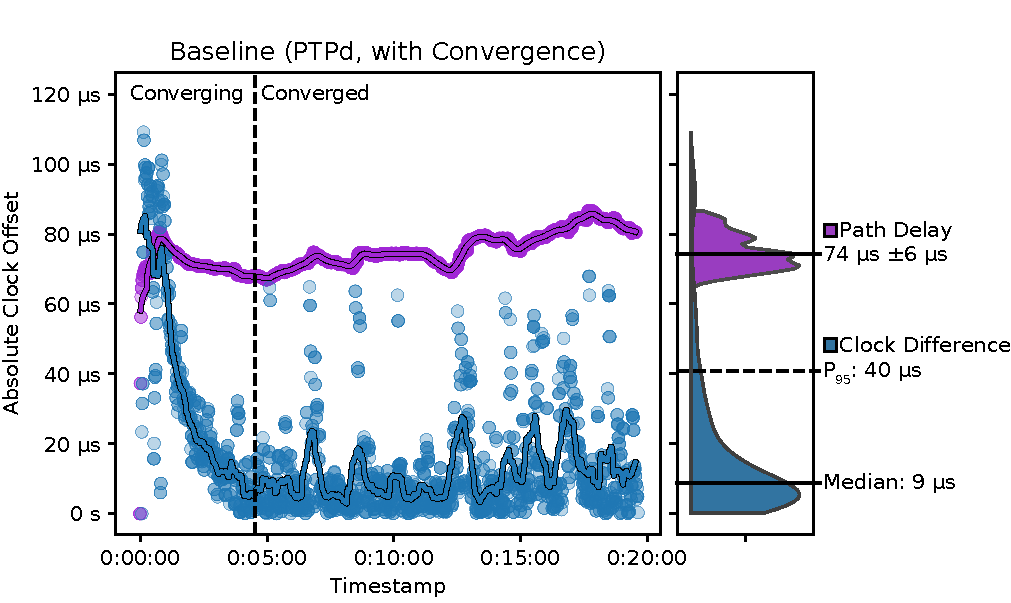
\includegraphics[width=\linewidth]{res/generated/base/rpi08-convergence_2.pdf}
    \caption{A sample run of LinuxPTP in its default configuration. Clock synchronization can follow different convergence trajectories, which needs to be accounted for when calculating statistics. Because PTP uses path delay compensation, the final clock synchronization accuracy is much better than the one-way path delay.}
    \label{fig:baseline_sample}
\end{figure}

Figure \ref{fig:baseline_sample} shows a sample run of the baseline for the PTPd vendor. In order to collect meaningful statistics, we apply some preprocessing to the collected profiles. The most important step is to remove the convergence phase (Figure \ref{fig:baseline_sample} left) from the profile to avoid it skewing the summary statistics. However, the clock travels on a different trajectory during each convergence, and a trajectory may include discontinuities, rebounds, and clock steps. To eliminate this unwanted data, we apply a heuristic to the raw clock offset (which can have positive or negative values depending on the offset direction): If the sign of the offset flips repeatedly over a specified window of time, this implies that there is no clear pattern to the measured offset that PTP can compensate for, and thus the clock offset is stable at its minimum value. Intuitively, this is somewhat equivalent to the average signed clock offset being zero, but note that the two are distinct for certain corner cases, as there are ways to produce an average zero clock offset that still exhibit a signal trend (which we want to avoid) and there can be measurement outliers that cause a non-zero average clock offset while showing no trend. Empirically, we find that using the frequency of sign switches in the clock offset produces much more accurate predictions of whether a clock is synchronized than relying on average (signed) offset.

\cmpSearchVendor{\ptpKey{base/rpi-4/\vendor/pd/q50}/\ptpKey{base/rpi-4/\vendor/q50}}
From Figure \ref{fig:baseline_sample} we observe that the clock offset is much lower than the corresponding path delay, due to the path delay compensation used by PTP clients. Across the tested vendors, we observe that the median absolute clock offset is between \fRatio{\cmpMin} (\fVendor{\cmpMinArg}) and \fRatio{\cmpMax} (\fVendor{\cmpMaxArg}) smaller than the magnitude of the path delay on the Raspberry-Pi 4 cluster,%
\cmpSearchVendor{\ptpKey{base/rpi-5/\vendor/pd/q50}/\ptpKey{base/rpi-5/\vendor/q50}}%
and \fRatio{\cmpMin} (\fVendor{\cmpMinArg}) to \fRatio{\cmpMax} (\fVendor{\cmpMaxArg}) smaller on the Raspberry-Pi 5 cluster, where hardware support is available.
Logically, the absolute clock difference exhibits some amount of skew due to the fact that the value cannot be negative, and the signal can experience bursts of noise which makes determining the true clock offset more difficult. Across the profile however, the median clock offset represents the best estimate of the real clock offset, while the 95\textsuperscript{th} percentile can be used as a bound where one can be reasonably sure that the true offset is lower.

\subsection{Vendors \& Systems}

\begin{figure}
    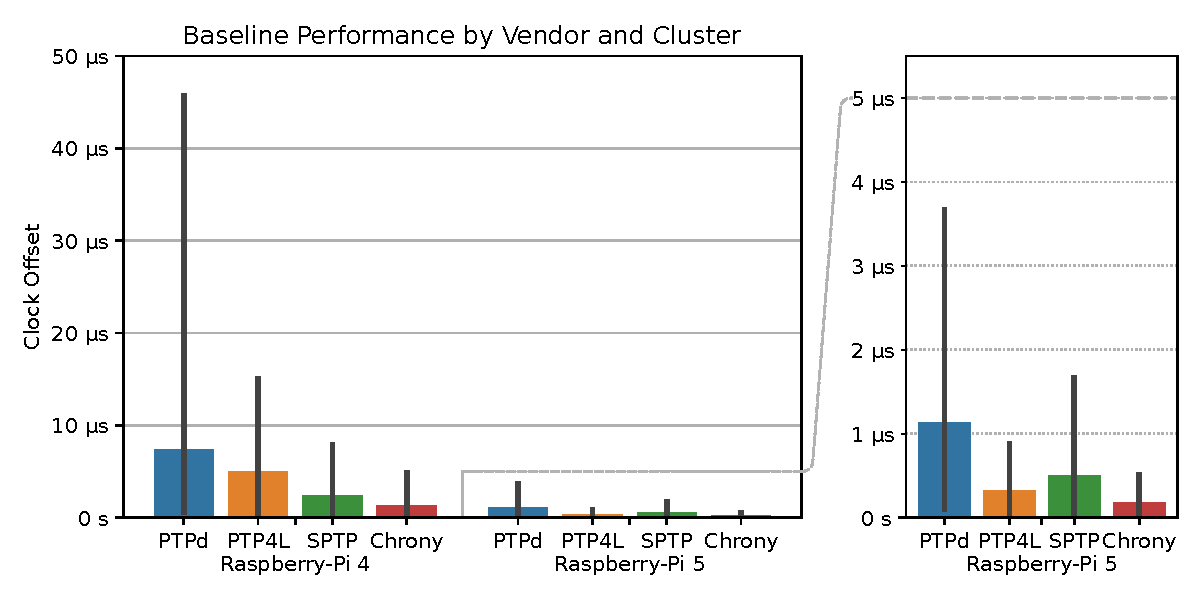
\includegraphics[width=\linewidth]{res/generated/base/vendor_comparison.pdf}
    \caption{Median baseline performance for all vendors, across our two hardware testbeds (left) and magnified for only the Raspberry-Pi 5 cluster (right). Error bands represent the 5\textsuperscript{th} and 95\textsuperscript{th} percentiles, respectively.}
    \label{fig:baseline}
\end{figure}

\begin{table}
\centering
\caption{Baseline Values by Vendor and System}

    \begin{tikzpicture}[start chain=rows going below, on grid, node distance=0.35cm and 2cm, text width=2cm, align=right]
        \node[on chain=rows] {};
        \begin{scope}[start branch=row going right]
            \node[on chain] {};
            \node[on chain] {Clock Offset};
            \node[on chain] {Clock Offset};
        \end{scope}

        \node[on chain=rows] {System};
        \begin{scope}[start branch=row going right]
            \node[on chain] {Vendor};
            \node[on chain] {Median};
            \node[on chain] {$P_{95}$};
        \end{scope}

            \foreach \system in {rpi-4,rpi-5}{
                \foreach  \vendor  in {ptpd,linuxptp,sptp,chrony}{
                    \node[on chain=rows] {\strcmpfullexpand{\vendor}{ptpd}{\fCluster{\system}}{}};

                    \begin{scope}[start branch=row going right]
                    \node[on chain] {\fVendor{\vendor}};
                    \node[on chain] {\fTimeKey[1]{base/\system/\vendor/q50}};
                    \node[on chain] {\fTimeKey{base/\system/\vendor/q95}};

                    \end{scope}
                }
            }
    \end{tikzpicture}
    \label{tbl:baseline}
\end{table}

\cmpSearchVendor{\ptpKey{base/rpi-5/\vendor/q50}}
\cmpSave{/ptpperf/cmp/base/rpi-5}
\cmpSearchVendor{\ptpKey{base/rpi-4/\vendor/q50}}
\cmpSave{/ptpperf/cmp/base/rpi-4}

% Best and worst vendors are the same
\assert{\ptpKey{cmp/base/rpi-4/minarg}}{\ptpKey{cmp/base/rpi-5/minarg}}
\assert{\ptpKey{cmp/base/rpi-4/maxarg}}{\ptpKey{cmp/base/rpi-5/maxarg}}


A logical first step is comparing each vendor's baseline across the systems. Figure~\ref{fig:baseline} shows the four vendors on the Raspberry-Pi 4 and Raspberry-Pi 5 clusters, with the precise values available in Table~\ref{tbl:baseline}. We observe that \fVendor{\cmpMaxArg} has the worst synchronization offset on both systems, with a median clock offset of \fTime[1]{\cmpMax} on the Raspberry-Pi 4 and \fTimeKey[1]{cmp/base/rpi-5/max} on the Raspberry-Pi 5.
\fVendor{\cmpMinArg}, on the other hand, has the best performance on both systems, with the clock offset estimate at just \fTime[1]{\cmpMin} and \fTimeKey[1]{cmp/base/rpi-5/min}, respectively.
\assert{\cmpMinArg}{chrony}%
That a regular NTP client can outperform all of our PTP clients might come as a surprise, with PTP being engineered specifically for precision, but Chrony is very much state-of-the-art and can take advantage of the same hardware acceleration that our PTP clients can while providing a lot more features.

\cmpSearchVendor{\ptpKey{base/rpi-4/\vendor/q50}/\ptpKey{base/rpi-5/\vendor/q50}}

The most noticeable effect on the synchronization quality is the hardware, which is expected since the Raspberry-Pi 5 offers hardware timestamping while the Raspberry-Pi 4 does not. The advantage ranges from \fRatio{\cmpMin} for \fVendor{\cmpMinArg} to \fRatio{\cmpMax} for \fVendor{\cmpMaxArg}. Curiously, although PTPd does not support hardware timestamping, it still offers around \fPercentage{\ptpKey{cmp/base/rpi-5/min}/\ptpKey{base/rpi-5/ptpd/q50}} of the performance of the top contender \fVendor{\ptpKey{cmp/base/rpi-5/minarg}}. While the difference is significant, it definitely falls short of an order of magnitude, showing that hardware timestamps alone are not a cure-all solution to clock-synchronization and cannot eliminate timing variations entirely.

%\todo{
%Advantages: \foreach \vendor in {ptpd,linuxptp,sptp,chrony}{\fRatio{\ptpKey{base/rpi-4/\vendor/q50}/\ptpKey{base/rpi-5/\vendor/q50}} }
%}

\cmpSearchVendor{\ptpKey{base/rpi-4/\vendor/q95}/\ptpKey{base/rpi-4/\vendor/q50}}%
Another aspect to notice is the difference between the median clock offset and the 95\textsuperscript{th} percentile. Without hardware support, this difference can be rather large and has a high spread (between \fRatio{\cmpMin} for the most stable vendor \fVendor{\cmpMinArg} and \fRatio{\cmpMax} for the least stable vendor \fVendor{\cmpMaxArg}),
whereas the magnitude is smaller when hardware support is offered on the Raspberry-Pi %
\cmpSearchVendor{\ptpKey{base/rpi-5/\vendor/q95}/\ptpKey{base/rpi-5/\vendor/q50}}%
(\fRatio[1]{\cmpMin} \fVendor{\cmpMinArg} -- \fRatio[1]{\cmpMax} \fVendor{\cmpMaxArg}).
This means that not only is the average performance improved, but the magnitude of outliers is reduced, which is especially important when considering the dependability aspect. For applications that need to rely on timing sources, this shows that hardware acceleration can make a significant impact, but of course this comes with the price tag associated with a more capable network interface.

\subsection{Reproducibility}
{

\pgfkeys{
    /reproducibility/rpi-4/.cd,
    ptpd/min/.initial={0.000005329},
    ptpd/median/.initial={0.000005976},
    ptpd/max/.initial={0.000024082},
    linuxptp/min/.initial={0.0000041995},
    linuxptp/median/.initial={0.0000049845},
    linuxptp/max/.initial={0.0000059645},
    sptp/min/.initial={0.000002234},
    sptp/median/.initial={0.000002448},
    sptp/max/.initial={0.0000027660000000000003},
    chrony/min/.initial={0.00000125},
    chrony/median/.initial={0.0000012990000000000002},
    chrony/max/.initial={0.0000014060000000000002},
}
\renewcommand{\ptpKeyPrefix}{/reproducibility/rpi-4}


\begin{figure}
    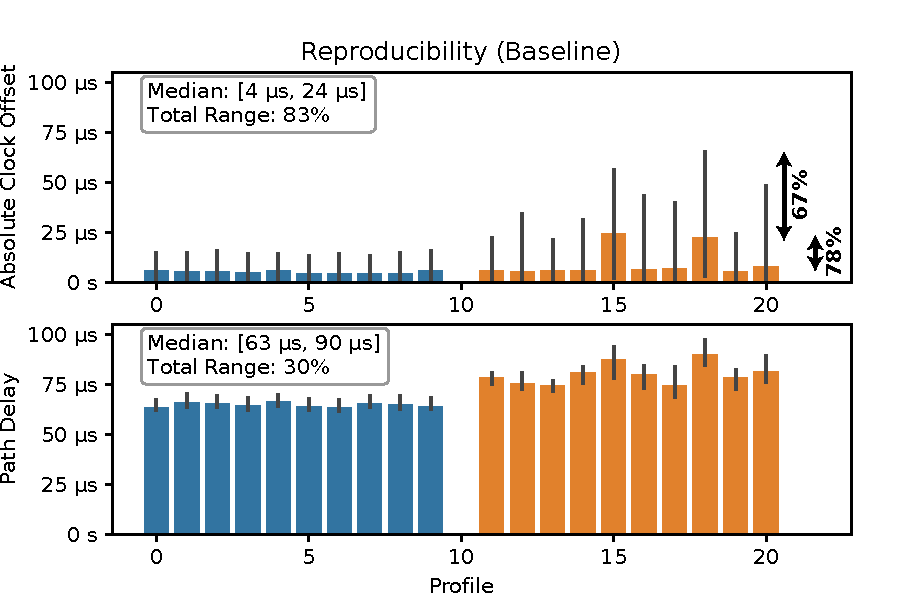
\includegraphics[width=\linewidth]{res/generated/base/key_metric_variance.pdf}
    \caption{Validating the baseline results by repeatedly measuring the baseline for both vendors on the Raspberry Pi 4 system. Top: The median absolute clock offset for each run, with error bars reaching from quantiles 0.05 to 0.95. Bottom: The same for the estimated path delay.}
    \label{fig:baseline_reproducibility}
\end{figure}

\newcommand{\numBaselineMeasurements}{10}
\newcommand{\baselineMinutesRuntime}{\numBaselineMeasurements*4*2*20}

The next question to be answered is how reproducible the measurement results are. Previously, all baseline results were aggregated into a single metric, but in reality the baseline consists of a number of independent measurements, which are measured interleaved for better compensation of noise that may be introduced through mechanisms outside our control. We repeated the measurement of the baseline observations ten times for each vendor on each hardware platform (totaling in around \fpeval{round(\baselineMinutesRuntime/60)} hours of runtime and \fpeval{round(\baselineMinutesRuntime*60)} samples collected) and aggregate them. Between each measurement run, the entire cluster is restarted to ensure that no state is carried over, which would harm the independence of observations. Otherwise, the setup is left untouched, so the only differences occur in the internal state of PTP.

\cmpSearchVendor{\ptpKey{\vendor/max}/\ptpKey{\vendor/min}}

Figure \ref{fig:baseline_reproducibility}\todo{Color scheme messed up on this one.} shows the results for two vendors, PTPd and LinuxPTP. We observe that LinuxPTP produces significantly more stable results for both the clock offset estimation and the path delay, while PTPd shows more variance in median and 95-th quantile observed clock offset, while additionally being less sure about the path delay. A simple restart of the PTP client can suddenly cause the median latency to jump from \fTimeKey{ptpd/min} up to \fTimeKey{ptpd/max}, which corresponds to an increase of \fRelative[-1]{\ptpKey{ptpd/max}/\ptpKey{ptpd/min}} not only momentarily, but throughout an entire run of 20 minutes. This already comes uncomfortably close to our safety factor of \safetyMargin, and we have not even started stressing the system yet. Fortunately, LinuxPTP produces a lot more stable results, with a smaller range of \fTimeKey{linuxptp/min} and \fTimeKey{linuxptp/max} between the best observed run and the worst observed run corresponding to just \fRelative{\ptpKey{linuxptp/max}/\ptpKey{linuxptp/min}} difference. The best vendor in this regard is \fVendor{\cmpMinArg} (not shown), with a range of just \fRelative{\cmpMin}, while the worst performance is observed with the aforementioned \fVendor{\cmpMaxArg}.
%
% Assert last sentence
\assert{\cmpMaxArg}{ptpd}
%
Needless to say, a vendor that cannot deliver stable timing guarantees is risky to deploy in a production environment that needs to rely upon the time source functioning. In the upcoming sections, we will examine whether PTP clients can be made resilient against potential external and internal influences.

}

\section{Resource Contention}

One aspect that influences how reliable PTP can operate is the outside interference originating from resource sharing. Through our research, we identified two key resources which need to be carefully managed so that PTP can provide synchronization even in the presence of stress: the network and the CPU.

\subsection{Network Contention}
\begin{figure}
    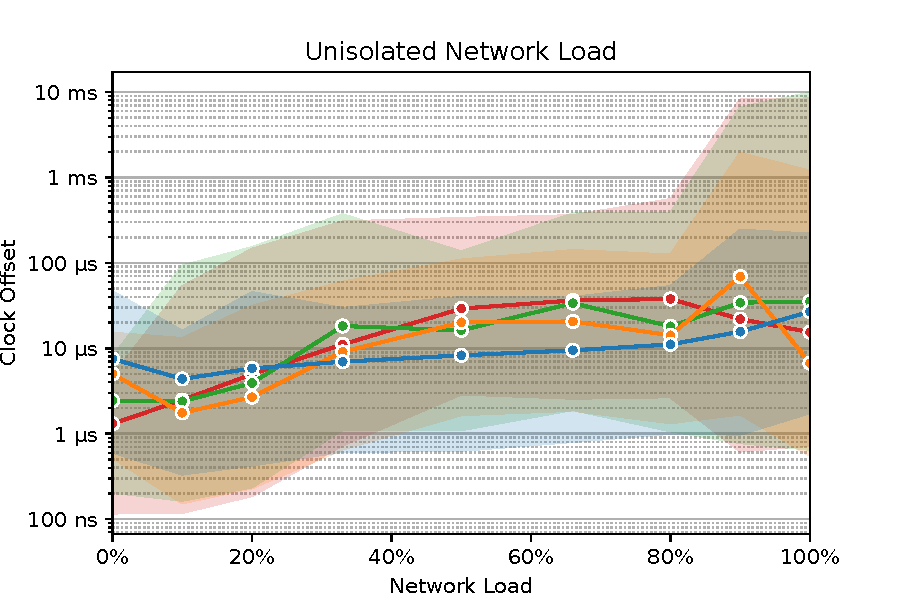
\includegraphics[width=\linewidth]{res/generated/net_unprioritized_trend_rpi-4.pdf}
    \caption{Clock synchronization accuracy at different levels of network load. All vendors experience degradation at higher network loads, though the degree to which they are affected differs. Apart from a change in median clock offset, the 95\textsuperscript{th} percentile is heavily affected, signaling larger and more frequent outliers.}
    \label{fig:network_load}
\end{figure}

\cmpSearchVendor{\ptpKey{load/net_unprioritized/load_100/rpi-4/\vendor/q50}/\ptpKey{base/rpi-4/\vendor/q50}}

Like stated previously, the synchronization accuracy principally depends on the magnitude and the variation of the path delay. Intuition therefore suggests that the more network load is present, the more PTP will struggle to measure the clock offset consistently due to increased queuing in software and hardware causing delay and delay variation in delivery. We simulate network load artificially using iPerf, a traffic generator that allows us to target our predefined data rates. By default, when a PTP vendor is installed on a target system and run, there are no special precautions in place to guard against contention, so a decrease in accuracy as the network load increases is exactly what we observe (Figure \ref{fig:network_load}). Interestingly, the vendor with the smallest increase in clock offset is \fVendor{\cmpMinArg}, with an increase of just \fRatio[1]{\cmpMin} (\fTimeKey{base/rpi-4/\cmpMinArg/q50} -- \fTimeKey{load/net_unprioritized/load_100/rpi-4/\cmpMinArg/q50}) from no network load to 100\% network load. On the other hand, \fVendor{\cmpMaxArg} has a much higher ratio of \fRatio{\cmpMax} (\fTimeKey{base/rpi-4/\cmpMaxArg/q50} -- \fTimeKey{load/net_unprioritized/load_100/rpi-4/\cmpMaxArg/q50}), which can only be partially attributed to the fact that \fVendor{\cmpMaxArg} has a smaller baseline value.
% Assert SPTP is worst
\assert{\cmpMaxArg}{sptp}%
SPTP is the only vendor that relies solely on unicast message exchange (a design choice by Meta), whether this is why SPTP appears to be more susceptible to contention is subject to further investigation.%
%
% 95-th percentiles
\cmpSearchVendor{\ptpKey{load/net_unprioritized/load_100/rpi-4/\vendor/q95}/\ptpKey{base/rpi-4/\vendor/q95}}%
The 95\textsuperscript{th} percentiles reflect the behavior of the outliers, and here we can observe even larger ranges, with \fVendor{\cmpMaxArg} now showing a ratio of \fRatio[-1]{\cmpMax} (\fTimeKey{base/rpi-4/\cmpMaxArg/q95} -- \fTimeKey[-1]{load/net_unprioritized/load_100/rpi-4/\cmpMaxArg/q95}). This is clearly above and beyond even very generous safety margins, so we need to examine how the effect of network load can be mitigated.

 Note that under network load PTP sometimes fails to synchronize at all, when it gets stuck in an infinite loop running into transmission timeouts and thus switching between ``state init'' and ``state faulty''. In this case the timing system breaks entirely, and no synchronization can be established at all. These measurements have been excluded from the shown data, but we encountered them rather frequently at high load levels. Preventing this is paramount, as having no synchronization is potentially a lot worse than having a bad quality signal.

\begin{figure}
    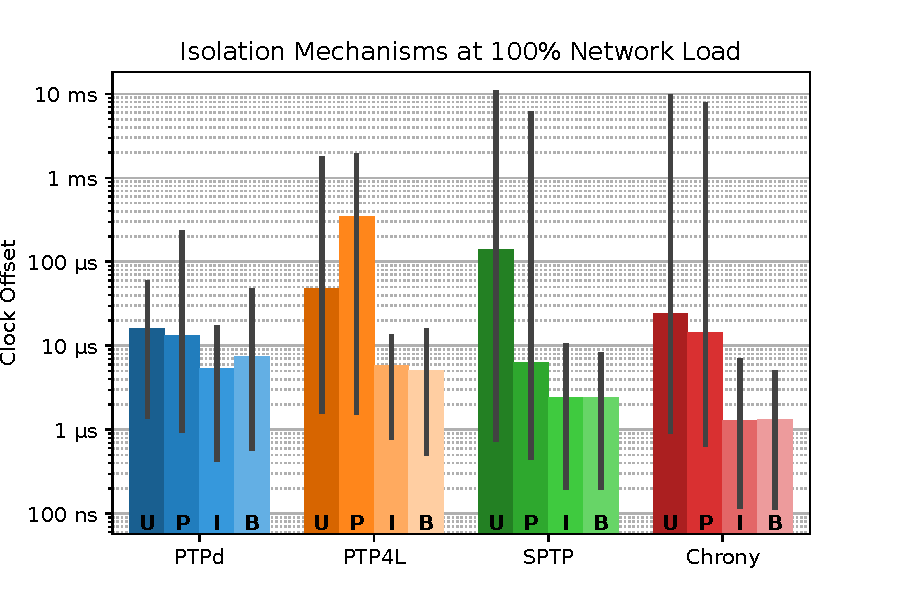
\includegraphics[width=\linewidth]{res/generated/net_isolation_comparison.pdf}
    \begin{center}
    \vspace{-0.5cm}
    \sffamily\scriptsize \textbf{U}: Unprioritized \quad\textbf{P}: Prioritized \quad\textbf{I}: Isolated \quad\textbf{B}: Baseline
    \end{center}
    \caption{Different possibilities of isolation network load, compared to the baseline with no load. Both prioritization and physical isolation can often improve performance over the unprioritized default, however only isolation can match the performance of the baseline without resource contention.}
    \label{fig:net_isolation_comparison}
\end{figure}

Depending on the possibility of dedicating exclusive resources to PTP, two principle solutions are viable: a software/hardware prioritization of traffic to reduce interference of lower priority traffic and providing a dedicated network interface for physical isolation. While the latter might seem like an expensive proposition and could therefore be less suited for embedded solutions, other use cases like industrial settings will often already provide a second management interface separate from the application's network. On our Raspberry-Pis, we emulate this by configuring the routing table so only PTP traffic can use the wired interface, with other traffic being relegated to the wireless interface. Figure~\ref{fig:net_isolation_comparison} shows these possibilities, with the default unisolated case on the left and the baseline on the very right.%
\cmpSearchVendor{\ptpKey{load/net_isolated/load_100/rpi-4/\vendor/q50}/\ptpKey{base/rpi-4/\vendor/q50}}%
%Worst: \fRatio[1]{\cmpMax} @ \cmpMaxArg{} and \fRatio[1]{\cmpMin} @ \cmpMinArg
\assertRange{\cmpMax}{1.0}{1.5}%
\assertRange{\cmpMin}{0.6}{1.0}%
Conforming to expectations, a physical isolation of PTP traffic can entirely mitigate the adverse effects of network load, with results sometimes even outperforming the baseline slightly (\fVendor{\cmpMinArg}: \fRelative{\cmpMin}, \fVendor{\cmpMaxArg}: \fRelative{\cmpMax}).
Theoretically, the only interference that could cross the isolation barrier is latency through cross-talk on the software network stack, which does not appear to be an issue here.
The software-only solution, however, cannot quite achieve the same level of performance on our testbed. Prioritization is achieved through differentiated services (via the Differentiated Services Code Point, DSCP), and requires prioritization support on every networking software and hardware component on the critical path to perform optimally. While our switch and operating system claim to support the technology, this does not appear to be sufficient for complete traffic segregation.
\cmpSearchVendor{\ptpKey{load/net_unprioritized/load_100/rpi-4/\vendor/q50}/\ptpKey{load/net_prioritized/load_100/rpi-4/\vendor/q50}}
Compared to no traffic prioritization, activating DSCP results in performance improvements up to \fRatio{\cmpMax} for \fVendor{\cmpMaxArg}.
However, one outlier exists, which is \fVendor{\cmpMinArg}, where the median vendor performance actually decreases by \fRatio{1/\cmpMin}, while the 5\textsuperscript{th} and 95\textsuperscript{th} percentiles remain the within 10\% of each other.
\assertRange{\cmpMin}{0.1}{0.2}
\assertRange{\ptpKey{load/net_unprioritized/load_100/rpi-4/linuxptp/q95}/\ptpKey{load/net_prioritized/load_100/rpi-4/linuxptp/q95}}{0.9}{1.1}
\assertRange{\ptpKey{load/net_unprioritized/load_100/rpi-4/linuxptp/q5}/\ptpKey{load/net_prioritized/load_100/rpi-4/linuxptp/q5}}{0.9}{1.1}
%
\newcommand{\numTrials}{min(\ptpKey{load/net_unprioritized/load_100/rpi-4/linuxptp/count}, \ptpKey{load/net_prioritized/load_100/rpi-4/linuxptp/count})}
We have examined the affected profiles in more detail and can confirm that this effect is visible on all \fNum{\numTrials} trials encompassing approximately \fNum{\numTrials * 20 * 60} samples, so while we are confident of the validity of the observation, the reason why it occurs is currently unknown.

\todo{Perhaps recommendations}

\subsection{Other shared resources}

\cmpSearchVendor{\ptpKey{load/cpu_unprioritized/load_100/rpi-4/\vendor/q50}/\ptpKey{base/rpi-4/\vendor/q50}}
We have examined the effect of contention on other shared resources, and fortunately none of them cause synchronization quality degradation at the level that network congestion does. For a fully loaded CPU, congestion causes a maximum observed median degradation of just \fRelative{\cmpMax} (\fVendor{\cmpMaxArg})%
\cmpSearchVendor{\ptpKey{load/cpu_unprioritized/load_100/rpi-4/\vendor/q95}/\ptpKey{base/rpi-4/\vendor/q95}}%
and \fRelative{\cmpMax} at the 95\textsuperscript{th} percentile, which is small enough not to make a practical difference.
\assert{\cmpMaxArg}{chrony}
TODO: What about \fRelative{\cmpMin} \fVendor{\cmpMinArg}?\todo{Determine}
Interestingly, some level of load can actually boost performance relative to the baseline (we observed this on both the CPU and the network).
We assume this occurs due to the hardware switching less into power saving states when more load is present, which may actually cause packets to be delivered faster.